\documentclass{article}
\usepackage[lmargin=2.54cm, rmargin=2.54cm,tmargin=2.54cm,bmargin=2.54cm]{geometry}
\usepackage{doc}
\usepackage{graphicx}
\usepackage{setspace}

\title{Music Software Usability Test}
\author{Anthony Menjivar}

\date{10/18/13}

\begin{document}

\maketitle

\abstract{

\section{Introduction}	
This is an experiment on three different music on three digital media software , used for playing, managing and organizing music media. These music libraries are used on computers, tablets and phones but for this study experimented on computers only. There will be three music software and they will be iTunes, Spotify and Google Music.  To gain data for this experiment we will have eight people, used as our test subjects, with completely random backgrounds on these three software, and computer software in general, go through three different tasks in each of the music libraries. All the tasks are able to be done in all three of the music libraries in order to make comparisons easier and better. Through these tasks they will be timed, recorded and asked questions to get the best data possible. With this we are trying to find the best  music libraries according to the data as well as what these people say. To measure which is the best, we will be using the five metrics of learnability, memorability, efficiency, errors and satisfaction. learnability, errors, and satisfation will be explicitly seen in the tests done, having a time, amount of errors, and satisfaction ratings. Further detail ill go into those metrics also. Memorability and Efficiency won't be explicit and will be discussed later and  will use what was calculated to see which is best with these two metrics.

We will go through what each task is as well as go through each test subject in detail to find reason behind the data collected. We then went over the total data collected after each task. 

This included asking the participants to rate how their satisfaction levels on each task they did out of 10 (10 being the best). Learnability will be the time taking to complete a task fully for participants with no prior experience of program.

\section{Task One}
The first task for the test subjects will be focused around creating three different playlists on each music library. Each subject will be asked to start off with one music library first and create all three playlists on that software before going onto the next one. The parameters to this first task for each subject are:


\begin{enumerate}
  \item Create a playlist
  \begin{enumerate}
    \item The playlist will contain two different artists
  \end{enumerate}
  \item Name the playlist with the names of the two artists
  \item Add 5 songs from each artist to the playlist
  \begin{enumerate}
    \item The playlist will contain a total of 10 songs 
  \end{enumerate}
  \item Repeat for two more playlists
  \begin{enumerate}
    \item There will be 30 songs in total with all three playlists
  \end{enumerate} 
\end{enumerate}

Subjects will be timed from the moment they start creating the playlist to when the playlist is completely finished. At the same time the subject will be timed to see how it takes to create all three playlists. While the subjects are creating the playlists, errors that they make will be recorded to give reason behind any differences of times.

(For the first participant, a small description will be given for each program to show details on what happened during the testing and the details pretty much are that same, more or less with the other participants. Therefore, the rest of the participants won't have these descriptions and each program will be talked about in general at the end of the report.) 

\begin{multicols}{2}
\subsection{1st Participant}
Background: This participant has used iTunes before. 

\subsubsection{\it iTunes}

This participant was told to create the three playlists using iTunes first. The participant took 2 minutes to create the first playlist completely. This participant did have an error in making a duplicate song in the playlist as he used a drag and drop technique to add songs to the playlist. The participant then took about 1 minute and 30 seconds to make the second playlist and the same to make the third. The reason behind this was his switch from the drag and drop technique to a command + click (Mac) technique where the participant was able to select all five of the songs at once and add them all at once into the playlist. Here is an overview of the metrics for this first task for the first participant:
\begin{itemize}
	\item {\bf Learnability:} N/A
	\item {\bf Errors:} 1
	\item {\bf Satisfaction:} 8 out of 10 
\end{itemize}

\subsubsection{\it Spotify}
The participant was then told to use Spotify. It took this participant 50 seconds to complete the first playlist. This difference could have come from him going straight to the technique where multiple songs can be added to the playlist. Because of this it also took 50 seconds each to complete the second and third playlist. The search bar had a lot to do with the speed of the playlists being created.
\begin{itemize}
	\item {\bf Learnability:} 2.5 minutes
	\item {\bf Errors:} None
	\item {\bf Satisfaction:} 10 out of 10 
\end{itemize}

\subsubsection{\it Google Music}
The participant then was told to use Google Music. It took the participant 5 minutes to create the playlists and it probably took the participant a little longer for the participant to create the playlists as they have never worked with an online music library like Google Music.
\begin{itemize}
\item {\bf Learnability:} 5 minutes
	\item {\bf Errors:} 1
	\item {\bf Satisfaction:} 6 out of 10 
\end{itemize}

	
\subsection{2nd Participant}
Background: This participant was not familiar with the three programs. This participant was introduced to the three programs to at least have some sort of idea.

\subsubsection{\it iTunes}
\begin{itemize}
	\item {\bf Learnability:} 8 minutes
	\item {\bf Errors:} 3
	\item {\bf Satisfaction:} 7 out of 10 
\end{itemize}

\subsubsection{\it Spotify}
\begin{itemize}
	\item {\bf Learnability:} 5 minutes
	\item {\bf Errors:} None
	\item {\bf Satisfaction:} 9 out of 10 
\end{itemize}

\subsubsection{\it Google Music}
\begin{itemize}
\item {\bf Learnability:} 10 minutes
	\item {\bf Errors:} 1
	\item {\bf Satisfaction:} 4 out of 10 
\end{itemize}
	
\subsection{3rd Participant}
Background: This participant was not familiar with any of these software. The participant was introduced to the three programs to at least have some sort of idea.

\subsubsection{\it iTunes}
\begin{itemize}
	\item {\bf Learnability:} 13 minutes
	\item {\bf Errors:} 4
	\item {\bf Satisfaction:} 8 out of 10 
\end{itemize}

\subsubsection{\it Spotify}
\begin{itemize}
	\item {\bf Learnability:} 11 minutes
	\item {\bf Errors:} None
	\item {\bf Satisfaction:} 7 out of 10 
\end{itemize}

\subsubsection{\it Google Music}
\begin{itemize}
\item {\bf Learnability:} 15 minutes
	\item {\bf Errors:}12
	\item {\bf Satisfaction:} 4 out of 10 
\end{itemize}

\subsection{4th Participant}
Background: This participant has had experience with using iTunes and Spotify.

\subsubsection{\it iTunes}
\begin{itemize}
	\item {\bf Learnability:} N/A
	\item {\bf Errors:} None
	\item {\bf Satisfaction:} 10 out of 10 
\end{itemize}

\subsubsection{\it Spotify}
\begin{itemize}
	\item {\bf Learnability:} N/A
	\item {\bf Errors:} None
	\item {\bf Satisfaction:} 9 out of 10 
\end{itemize}

\subsubsection{\it Google Music}
\begin{itemize}
\item {\bf Learnability:} 3 minutes
	\item {\bf Errors:}None
	\item {\bf Satisfaction:} 7 out of 10 
\end{itemize}

\subsection{5th Participant}
Background: Experience with iTunes before

\subsubsection{\it iTunes}
\begin{itemize}
	\item {\bf Learnability:} N/A
	\item {\bf Errors:} 1
	\item {\bf Satisfaction:} 9 out of 10 
\end{itemize}

\subsubsection{\it Spotify}
\begin{itemize}
	\item {\bf Learnability:} 5 minutes
	\item {\bf Errors:} 2
	\item {\bf Satisfaction:} 7 out of 10 
\end{itemize}

\subsubsection{\it Google Music}
\begin{itemize}
\item {\bf Learnability:} 5 minutes
	\item {\bf Errors:}1
	\item {\bf Satisfaction:} 8 out of 10 
\end{itemize}  

\subsection{6th Participant}
Background: Knowledge with all three programs

\subsubsection{\it iTunes}
\begin{itemize}
	\item {\bf Learnability:} N/A
	\item {\bf Errors:} 1
	\item {\bf Satisfaction:} 6 out of 10 
\end{itemize}

\subsubsection{\it Spotify}
\begin{itemize}
	\item {\bf Learnability:} N/A
	\item {\bf Errors:} 1
	\item {\bf Satisfaction:} 7 out of 10 
\end{itemize}

\subsubsection{\it Google Music}
\begin{itemize}
\item {\bf Learnability:} N/A
	\item {\bf Errors:}None
	\item {\bf Satisfaction:} 10 out of 10 
\end{itemize}  
\subsection{7th Participant}
Background: Experience with iTunes before

\subsubsection{\it iTunes}
\begin{itemize}
	\item {\bf Learnability:} N/A
	\item {\bf Errors:} 1
	\item {\bf Satisfaction:} 9 out of 10 
\end{itemize}

\subsubsection{\it Spotify}
\begin{itemize}
	\item {\bf Learnability:} 4.5 minutes
	\item {\bf Errors:} 2
	\item {\bf Satisfaction:} 8 out of 10 
\end{itemize}

\subsubsection{\it Google Music}
\begin{itemize}
\item {\bf Learnability:} 5 minutes
	\item {\bf Errors:}1
	\item {\bf Satisfaction:} 7 out of 10 
\end{itemize} 

\subsection{8th Participant}
Background: Experience with iTunes before

\subsubsection{\it iTunes}
\begin{itemize}
	\item {\bf Learnability:} N/A
	\item {\bf Errors:} 1
	\item {\bf Satisfaction:} 9 out of 10 
\end{itemize}

\subsubsection{\it Spotify}
\begin{itemize}
	\item {\bf Learnability:} 5 minutes
	\item {\bf Errors:} 2
	\item {\bf Satisfaction:} 7 out of 10 
\end{itemize}

\subsubsection{\it Google Music}
\begin{itemize}
\item {\bf Learnability:} 5 minutes
	\item {\bf Errors:}1
	\item {\bf Satisfaction:} 7 out of 10 
\end{itemize} 
\end{multicols}

\section{Task Two}
The object of the second task is for the participants to search for 5 different songs on the online store of each program. They are required to first go into the store and in any way that they want to or may know to look for songs they may use to find them. Time was stopped once the participant clicked on the song to denote it was founded. 

\begin{multicols}{2}
\subsection{1st Participant}

\subsubsection{\it iTunes}
This participant didn’t take too long to understand the iTunes store. It took this user 55 seconds to find the first song and then 35 seconds to find each of the other four songs. 
\begin{itemize}
	\item {\bf Learnability:} N/A
	\item {\bf Errors:}  None
	\item {\bf Satisfaction:} 9 out of 10 
\end{itemize}

\subsubsection{\it Spotify}
For the participant it took 20 seconds to find each song. It was much quicker than iTunes to an extent because the store search bar is already on the program.
\begin{itemize}
	\item {\bf Learnability:} 1.66 minutes
	\item {\bf Errors:} None
	\item {\bf Satisfaction:} 10 out of 10 
\end{itemize}

\subsubsection{\it Google Music}
Google Music was a little trickier for the participant. The main error was that this participant was searching in the wrong place instead of the store and took a while to figure that out. Once the actual search was figured out the songs took 30 seconds to find but it took 3 minutes to figure out the “Shop” in Google Music.
\begin{itemize}
\item {\bf Learnability:} 5.5 minutes
	\item {\bf Errors:}5
	\item {\bf Satisfaction:} 7 out of 10 
\end{itemize} 

\subsection{2nd Participant}

\subsubsection{\it iTunes}
\begin{itemize}
	\item {\bf Learnability:} 6 minutes
	\item {\bf Errors:}  3
	\item {\bf Satisfaction:} 6 out of 10 
\end{itemize}

\subsubsection{\it Spotify}
\begin{itemize}
	\item {\bf Learnability:} 4 minutes
	\item {\bf Errors:} None
	\item {\bf Satisfaction:} 10 out of 10 
\end{itemize}

\subsubsection{\it Google Music}
\begin{itemize}
\item {\bf Learnability:} 5.5 minutes
	\item {\bf Errors:}4 
	\item {\bf Satisfaction:} 5 out of 10 
\end{itemize}

\subsection{3rd Participant}

\subsubsection{\it iTunes}
\begin{itemize}
	\item {\bf Learnability:} 5 minutes
	\item {\bf Errors:}  2
	\item {\bf Satisfaction:} 9 out of 10 
\end{itemize}

\subsubsection{\it Spotify}
\begin{itemize}
	\item {\bf Learnability:} 3 minutes
	\item {\bf Errors:} None
	\item {\bf Satisfaction:} 10 out of 10 
\end{itemize}

\subsubsection{\it Google Music}
\begin{itemize}
\item {\bf Learnability:} 15 minutes
	\item {\bf Errors:} 13
	\item {\bf Satisfaction:} 3 out of 10 
\end{itemize}

\subsection{4th Participant}

\subsubsection{\it iTunes}
\begin{itemize}
	\item {\bf Learnability:} N/A
	\item {\bf Errors:}  None
	\item {\bf Satisfaction:} 10 out of 10 
\end{itemize}

\subsubsection{\it Spotify}
\begin{itemize}
	\item {\bf Learnability:} N/A
	\item {\bf Errors:} None
	\item {\bf Satisfaction:} 10 out of 10 
\end{itemize}

\subsubsection{\it Google Music}
\begin{itemize}
\item {\bf Learnability:} 4 minutes
	\item {\bf Errors:} None
	\item {\bf Satisfaction:} 8 out of 10 
\end{itemize}

\subsection{5th Participant}

\subsubsection{\it iTunes}
\begin{itemize}
	\item {\bf Learnability:} N/A
	\item {\bf Errors:}  3
	\item {\bf Satisfaction:} 9 out of 10 
\end{itemize}

\subsubsection{\it Spotify}
\begin{itemize}
	\item {\bf Learnability:} 1 minute
	\item {\bf Errors:} None
	\item {\bf Satisfaction:} 7 out of 10 
\end{itemize}

\subsubsection{\it Google Music}
\begin{itemize}
\item {\bf Learnability:} .75 minutes
	\item {\bf Errors:} None
	\item {\bf Satisfaction:} 8 out of 10 
\end{itemize}

\subsection{6th Participant}

\subsubsection{\it iTunes}
\begin{itemize}
	\item {\bf Learnability:} N/A
	\item {\bf Errors:}  None
	\item {\bf Satisfaction:} 6 out of 10 
\end{itemize}

\subsubsection{\it Spotify}
\begin{itemize}
	\item {\bf Learnability:} N/A
	\item {\bf Errors:} None
	\item {\bf Satisfaction:} 7 out of 10 
\end{itemize}

\subsubsection{\it Google Music}
\begin{itemize}
\item {\bf Learnability:} N/A minutes
	\item {\bf Errors:} None
	\item {\bf Satisfaction:} 10 out of 10 
\end{itemize}

\subsection{7th Participant}

\subsubsection{\it iTunes}
\begin{itemize}
	\item {\bf Learnability:} N/A
	\item {\bf Errors:}  None
	\item {\bf Satisfaction:} 9 out of 10 
\end{itemize}

\subsubsection{\it Spotify}
\begin{itemize}
	\item {\bf Learnability:} 1 minutes
	\item {\bf Errors:} None
	\item {\bf Satisfaction:} 8 out of 10 
\end{itemize}

\subsubsection{\it Google Music}
\begin{itemize}
\item {\bf Learnability:} .66 minutes
	\item {\bf Errors:} 1
	\item {\bf Satisfaction:} 7 out of 10 
\end{itemize}

\subsection{8th Participant}

\subsubsection{\it iTunes}
\begin{itemize}
	\item {\bf Learnability:} N/A
	\item {\bf Errors:} None
	\item {\bf Satisfaction:} 9 out of 10 
\end{itemize}

\subsubsection{\it Spotify}
\begin{itemize}
	\item {\bf Learnability:} 1 minutes
	\item {\bf Errors:} None
	\item {\bf Satisfaction:} 7 out of 10 
\end{itemize}

\subsubsection{\it Google Music}
\begin{itemize}
\item {\bf Learnability:} .833 minutes
	\item {\bf Errors:} None
	\item {\bf Satisfaction:} 7 out of 10 
\end{itemize}
\end{multicols}

\section{Task Three}
The third task consists of importing a folder with 10 different songs from an existing local folder to the programs themselves. The time for this task will be stopped once all 10 songs have been imported into their respective programs.

\begin{multicols}{2}
\subsection{1st Participant}

\subsubsection{\it iTunes}
This participant used iTunes first and easily found the “Add to Library” and was able to import the songs quickly.
\begin{itemize}
	\item {\bf Learnability:} N/A
	\item {\bf Errors:}  None
	\item {\bf Satisfaction:} 10 out of 10 
\end{itemize}

\subsubsection{\it Spotify}
The participant used Spotify second and found it a bit more complicated. It was harder to find how to import the songs for this user. Once the user found out how it’s done the task was completed in 7 minutes.
\begin{itemize}
	\item {\bf Learnability:} 7 minutes
	\item {\bf Errors:} None
	\item {\bf Satisfaction:} 6 out of 10 
\end{itemize}

\subsubsection{\it Google Music}
Google Music was very complicated for this user. It is not clear at all how to add music to the program for this user. Errors were committed mostly to try and find how it is music is imported. Once it was figured out, the user took 20 minutes to do all the work.
\begin{itemize}
\item {\bf Learnability:} 20 minutes
	\item {\bf Errors:} 15
	\item {\bf Satisfaction:} 2 out of 10 
\end{itemize} 

\subsection{2nd Participant}

\subsubsection{\it iTunes}
\begin{itemize}
	\item {\bf Learnability:} 1 minutes
	\item {\bf Errors:}  None
	\item {\bf Satisfaction:} 10 out of 10 
\end{itemize}

\subsubsection{\it Spotify}
\begin{itemize}
	\item {\bf Learnability:} 8 minutes
	\item {\bf Errors:} 3
	\item {\bf Satisfaction:} 6 out of 10 
\end{itemize}

\subsubsection{\it Google Music}
\begin{itemize}
\item {\bf Learnability:} 14 minutes
	\item {\bf Errors:} 8
	\item {\bf Satisfaction:} 3 out of 10 
\end{itemize}

\subsection{3rd Participant}

\subsubsection{\it iTunes}
\begin{itemize}
	\item {\bf Learnability:} 3 minutes
	\item {\bf Errors:}  None
	\item {\bf Satisfaction:} 10 out of 10 
\end{itemize}

\subsubsection{\it Spotify}
\begin{itemize}
	\item {\bf Learnability:} 8 minutes
	\item {\bf Errors:} 3
	\item {\bf Satisfaction:} 6 out of 10 
\end{itemize}

\subsubsection{\it Google Music}
\begin{itemize}
\item {\bf Learnability:} 28 minutes
	\item {\bf Errors:} 16
	\item {\bf Satisfaction:} 1 out of 10 
\end{itemize}

\subsection{4th Participant}

\subsubsection{\it iTunes}
\begin{itemize}
	\item {\bf Learnability:} N/A
	\item {\bf Errors:}  None
	\item {\bf Satisfaction:} 10 out of 10 
\end{itemize}

\subsubsection{\it Spotify}
\begin{itemize}
	\item {\bf Learnability:} N/A
	\item {\bf Errors:} None
	\item {\bf Satisfaction:} 10 out of 10 
\end{itemize}

\subsubsection{\it Google Music}
\begin{itemize}
\item {\bf Learnability:} 10 minutes
	\item {\bf Errors:} 4
	\item {\bf Satisfaction:} 6 out of 10 
\end{itemize}

\subsection{5th Participant}

\subsubsection{\it iTunes}
\begin{itemize}
	\item {\bf Learnability:} N/A
	\item {\bf Errors:}  None
	\item {\bf Satisfaction:} 9 out of 10 
\end{itemize}

\subsubsection{\it Spotify}
\begin{itemize}
	\item {\bf Learnability:} 1 minute
	\item {\bf Errors:} 1
	\item {\bf Satisfaction:} 7 out of 10 
\end{itemize}

\subsubsection{\it Google Music}
\begin{itemize}
\item {\bf Learnability:} 33 minutes
	\item {\bf Errors:} None
	\item {\bf Satisfaction:} 8 out of 10 
\end{itemize}

\subsection{6th Participant}

\subsubsection{\it iTunes}
\begin{itemize}
	\item {\bf Learnability:} N/A
	\item {\bf Errors:}  None
	\item {\bf Satisfaction:} 6 out of 10 
\end{itemize}

\subsubsection{\it Spotify}
\begin{itemize}
	\item {\bf Learnability:} N/A
	\item {\bf Errors:} None
	\item {\bf Satisfaction:} 7 out of 10 
\end{itemize}

\subsubsection{\it Google Music}
\begin{itemize}
\item {\bf Learnability:} N/A minutes
	\item {\bf Errors:} None
	\item {\bf Satisfaction:} 10 out of 10 
\end{itemize}

\subsection{7th Participant}

\subsubsection{\it iTunes}
\begin{itemize}
	\item {\bf Learnability:} N/A
	\item {\bf Errors:}  None
	\item {\bf Satisfaction:} 9 out of 10 
\end{itemize}

\subsubsection{\it Spotify}
\begin{itemize}
	\item {\bf Learnability:}  .6 minute
	\item {\bf Errors:} None
	\item {\bf Satisfaction:} 8 out of 10 
\end{itemize}

\subsubsection{\it Google Music}
\begin{itemize}
\item {\bf Learnability:} .5 minutes
	\item {\bf Errors:} 1
	\item {\bf Satisfaction:} 7 out of 10 
\end{itemize}

\subsection{8th Participant}

\subsubsection{\it iTunes}
\begin{itemize}
	\item {\bf Learnability:} N/A
	\item {\bf Errors:} None
	\item {\bf Satisfaction:} 9 out of 10 
\end{itemize}

\subsubsection{\it Spotify}
\begin{itemize}
	\item {\bf Learnability:} .16 minutes
	\item {\bf Errors:} None
	\item {\bf Satisfaction:} 7 out of 10 
\end{itemize}

\subsubsection{\it Google Music}
\begin{itemize}
\item {\bf Learnability:} .5 minutes
	\item {\bf Errors:} None
	\item {\bf Satisfaction:} 7 out of 10 
\end{itemize}
\end{multicols}

\section{Usability Metrics Overview}
We have numbers here from all the participants going through the tasks. With these numbers we can give an overview of how each of these five stacks up and how each program compares with one another.

\subsection{Learnability}
Learnability was taken down as the time it took for a participant to complete a task fully on each program. Many participants had knowledge of one or more of the programs, therefore there was no learnability to be counted for those particpants and those programs. For those that had no experience. We went through each task, each program and the calculations to see which had the best results when it came down to completing each task quickly.

\begin{center}
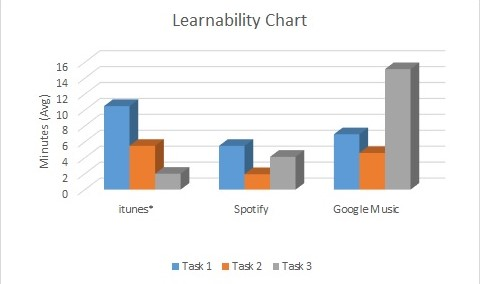
\includegraphics[width=120mm]{Learnability.jpg}
\end{center}
\begin{center}
Figure 1: Average comparison for Learnability (*The numbers for iTunes in this chart are very skewed as only two participants have never used the program before the test.
\end{center}

\subsection{Errors}
Errors were taken down as the participant went through wrong parts of the program or just clicked on wrong things and things of that nature. We went through each task, saw how many errors, calculated the average of each and compared each of the programs when it came to errors. This will show which program is the most error prone and in this case a higher number means it's worse.

\begin{center}
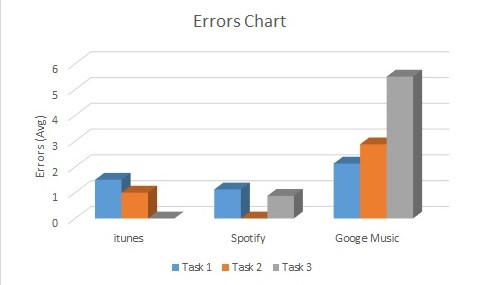
\includegraphics[width=120mm]{Errors.jpg}
\end{center}
\begin{center}
Figure 1: Average comparison for Errors in each program
\end{center}

\subsection{Satisfaction}
After each task done with all three programs we asked the participant to rate the program to their liking on a scale of 1-10 (10 being the highest). We did the same thing here and got the numbers, averaged them out and compared them side by side to see which program was the most satisfactory to users.

\begin{center}
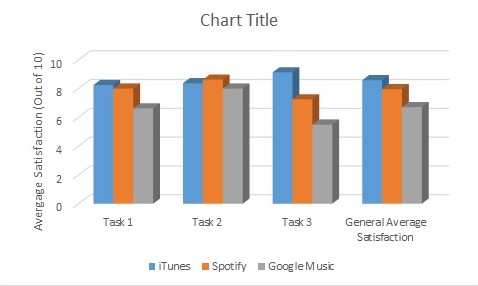
\includegraphics[width=120mm]{Satisfaction.jpg}
\end{center}
\begin{center}
Figure 1: Average comparison of Satisfaction for each program (Included is an overall satisfaction average)
\end{center}

\subsection{Efficiency}
Efficiency was not so explicit when it came to numbers in these tests done with the 8 participants.
\subsection{Memorability}
Memorability was  also not so explicit when it came to numbers in these tests done with the 8 participants.
\section{Conclusion}
According to what we see here we can see how each program was interacted with and which program seems to be better for what and the overall better program.

We see that a lot of users that weren’t familiar with the programs went through a lot of the program to try and figure out what was where in order to get the tasks done, which is the learnability portion.  Through these interactions with the programs, some participants looked at the programs differently and got a different feel for it, which might have caused there to be different satisfaction levels.

In the study we get to see that iTunes and Spotify were seen as the best options in between the test studies as well as the most satisfactory. iTunes maybe gets a bit over the lead here where there are more people that have used iTunes because it is a little more popular. Google Music isn’t really seen as that great because of the fact that it is different. Google Music is a cloud program instead of an application program which made it difficult for people to understand it and therefore not like it as much as the others.

\end{document} 